\documentclass{article}
\usepackage[utf8]{inputenc}
\usepackage[a4paper, total={6in, 8in}]{geometry}
\usepackage{graphicx}
\title{Analysis of price variation of different commodities in various Maharashtra Mandis}
\author{Vipul Joshi }
\date{March 2019}
\graphicspath{{C:/Users/vipul/Documents/Github/maharashtra_mandi/figures/}}
\begin{document}
   


\maketitle
 \begin{abstract}
        A discussion on the methodology followed to clean, visualise and model monthly price variation of various crops for the case of Mandis in Maharashtra has been presented. In order to be able to understand the trends in the mandi prices for different commodities, the presented dataset was first checked for inconsistencies like missing values, inconsistent usage of case for words, outliers etc. This was followed by visual inspection of the effect of cleaning stage to make sure that the anomalies has been adequately captured. The "cleaned" file generated at this stage was then used to generate an "overall" trend for each commodity across all the mandis. It was realised that the method of removal of the overall trend would be dependent on the seasonality type i.e. additive or multiplicative. Both the methods were used to remove the overall trend and to obtain the residuals. The residuals were inspected upon by spectral analysis as well as Augmented Dickey-Fuller test. The tests suggested that the modal prices across the mandis are affected by multiplicative seasonality. Further, the overall trend was decomposed into a linear trend and a seasonal trend. The coefficients for all the commodities (averaged over all the mandis) were found by a simple linear curve fitting and saved into a file for further processing. It may be noted that although the analysis was done for each commodity, onion was chosen to show the results. The details of the methodology are presented in the present document. Of particular interest is the onion price volatility. The prices are affected by a numerous factors including unpredictable behavior, hoarding practices, intermediaries involved in the distribution of quantity etc. 
    \end{abstract}
\section{Methodology}
\subsection{Data Cleaning}
The presented challenge was about understanding the price variation of commodities across the mandis in Maharashtra. The provided dataset "Monthly data cmo.csv" contained sequential information about the maximum, minimum and modal prices of the variety of commodities. Along with the aforementioned information, the quantity arriving across the mandis of Maharashtra was also provided. Upon importing the dataset into the Jupyter notebook, dataset was checked for inconsistencies. Although there were no missing values in the dataset, categorical features were found to be improperly cased. Data of all the categorical features was transformed into lower case. As the dataset contained information for different commodities, it was realised that the overall description might not provide an accurate insight into the statistics of the data. Therefore, the dataset was grouped into different commodities and then inspected for outliers. Outliers were identified as points which did not lie between $[QR1-3.0*IQR, QR3+3.0*IQR]$, where $QR1$ is the first quartile, $QR3$ is the third quartile and $IQR$ is the inter-quartile range. The outliers were replaced with $QR3$ values of the group (instead of replacing the outliers with mean of the group). In the meanwhile, group statistics showed that some of the commodities had only one degree of freedom i.e. contained only a single sample point and were removed.The processed data was then saved into another Comma Separated Values (CSV) file for post-processing.
\subsection{Seasonality Test of Modal Prices}
A time series typically consists of following components: \\
1. Trend component: long-run increase or decrease of the values in the time-series. \\
2. Seasonal component: quarterly or monthly variation in the values of the time-series depending on the time of the year \\
3. Cyclic component: business or economic effect on the values.  \\
4. Irregular components: random variations due to unpredictable events. \\
One or more of the above mentioned components may be present in the time-series. One of the objective of the present challenge was to identify trend and seasonality in the data. In order to decompose the data into these components, a series (containing time-varying data) may be represented by either of the following: \\
\begin{equation}\label{multiplicative}
    f(t) = S(t)*Tr(t)*Cyc(t)*Irr(t)
\end{equation}
\begin{equation} \label{additive}
    f(t) = S(t)+Tr(t)+Cyc(t)+Irr(t)
\end{equation}
where $f(t)$ is the time-series and $S(t), \, Cyc(t), \& Irr(t)$ are the seasonal, cyclic and irregular components. Eq. \ref{multiplicative} and Eq. \ref{additive} are the multiplicative and additive representations of the time series. \\
The objective of the seasonality test was to identify the type of seasonality and to de-seasonalise the data. Since the data was collected in discrete intervals (one-month), trend and seasonality were removed in a combined fashion in form of the moving average (averaged over month for individual commodity). The moving average was first subtracted from the data and its effect on mean and standard deviation was noticed. It was observed that the mean was reduced to zero while the standard deviation remained unaffected. This suggested that the seasonality may not be additive. Fourier Transform of the residuals showed sharp peaks at the period of the season. This suggested that the seasonality has not been removed. \\
In the second stage, the data was divided by the moving average. The mean and the standard deviation of the residuals were reduced to minimum in the process. This suggested that the data has been rendered stationary. In order to verify, the residuals in the time-domain were transformed into frequency-domain via Fourier Transform. The fundamental as well as all the harmonics of the power spectral density were suppressed by a factor of over $10^{15}$. Therefore, it was concluded that the seasonality is of multiplicative type.
\subsection{Trend Analysis}
In the previous section, it was argued that the seasonality is of multiplicative type and it was removed by dividing the time series by moving average. This means that the moving average must contain the trend and seasonal components. Earlier, the entire dataset was grouped by commodity and aggregated by mean over all the mandis. In order to extract the trend for all the commodities, linear regression was used to obtain the intercept, slope and $r^2$ for each of them. In this case, it was interesting to note that the $r^2$ value was lower for seasonal crops. This helped in identifying the crops that have seasonal behavior and was analysed using periodogram for some selective cases. The intercept, slope and $r^2$ have been saved into a file. 
\section{Analysis of commodity prices}
Agriculture is one the most important factor in Maharashtra's economy. According to Wikipedia, agriculture contributes to almost $ 12\% $ GDP by sector for India. Principle crops grown in the state are rice, jowar, wheat, tur, gram etc. The state is also one of the largest producer of onion in the country. As per a report by Union Budget and Economic Survey, Ministry of Finance, Maharashtra was ranked first in production of pulses, second in production of cereals, sugarcane, soyabean, cotton and third in sunflower in 2007. It is also obvious that the local prices of these commodities would dictate the national prices. A timeline of interest in the agricultural sector of Maharashtra is from 2013-2016 in which agriculture exports from Maharashtra took a hard hit. According to an article published on March 2015, the onion exports had dropped by over 100\%.  Other commodities like grapes and pulses saw a 40\% dip. The loss in the agricultural products was attributed to unseasonal rains which damaged onion seed plots in the state. Another reason that this timeline is important is because the sate recovered quickly and the prices were first stabilised and then hit a rock bottom in January 2016. The intervention by the State Government with a decision to slash the minimum export price. The arrival of the commodity had increased due to record breaking sowing of the plant. \par
\begin{figure*} 
	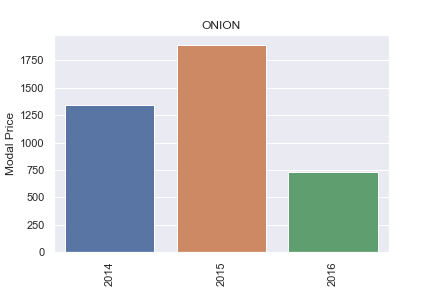
\includegraphics[width=7cm,height=7cm]{onion_yearly.png}
	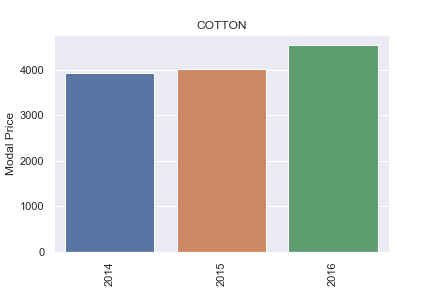
\includegraphics[width=7cm,height=7cm]{cotton_yearly.png}\\
	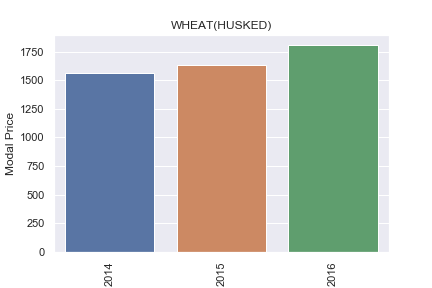
\includegraphics[width=7cm,height=7cm]{wheat(husked)_yearly.png}
	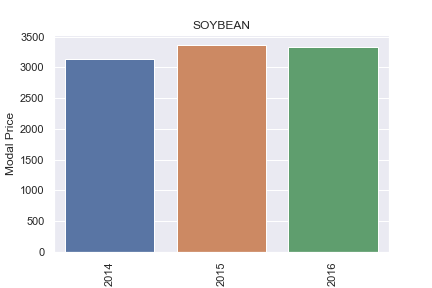
\includegraphics[width=7cm,height=7cm]{soybean_yearly.png}
	\caption{Yearly price variation of onion, cotton,}
	\label{fig:Yearly}
\end{figure*}
\begin{figure*}
	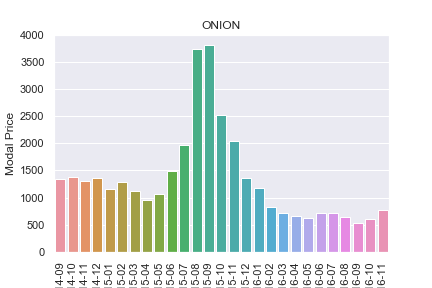
\includegraphics[width=8cm,height=7cm]{onion_monthly.png}
	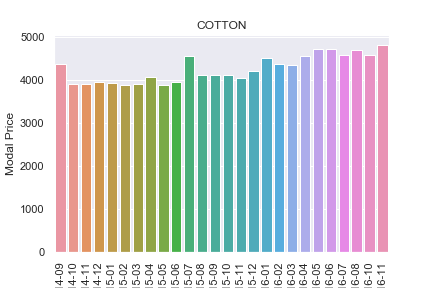
\includegraphics[width=8cm,height=7cm]{cotton_monthly.png}\\
	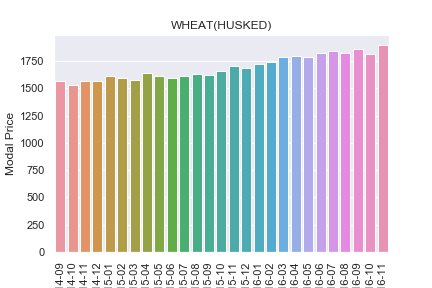
\includegraphics[width=8cm,height=7cm]{wheat(husked)_monthly.png}
	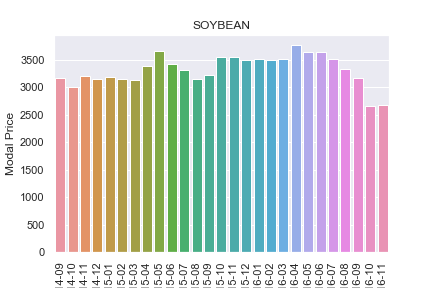
\includegraphics[width=8cm,height=7cm]{soybean_monthly.png}
	\caption{Monthly price variation of onion, cotton,}
	\label{fig:month}
\end{figure*}
The dataset available for analysis contains information about the price variation of 352 commodities across 349 Agricultural Produce Market Committee (APMC) for time between 2014 to 2016. The available dataset captures the seasonal modal price variations in the above mentioned time period and is therefore a rich dataset to perform time series analysis. As mentioned above, the important crops produced in Maharashtra are wheat, soyabean, cotton, onion etc. Fig. \ref{fig:Yearly} shows the price variation of these crops as a function of years. These figures give a very "neat" picture of the price variation. Although the price rise over years is expected; however the prices of onion was substantially higher in 2015 and  lower in 2016 . A granular look (Fig. \ref{fig:month}) into the price variation will reveal that onion prices were infact affected by the unseasonal rains and its effect was seen in the month of September 2015. These two graphs are indicative of the seasonal component (as seen in the monthly price fluctuation of onion) and trend component (as seen in the annual price variation of cotton or wheat). The objective of the document is to bring out these components from the available data. It was already mentioned that the seasonal component of the commodity prices is represented by $S(t)$. The frequency of the season may be found out by the following equation:
\begin{equation}
 F(\omega) = \int_{-\infty}^{\infty}S(t)S^*(t)\exp(-i\omega t)dt
\end{equation}
where $F(\omega)$ is the frequency domain expression of $S(t)$, $S^*(t)$ is the complex conjugate of the time-series. An important point to note is that the above mentioned tranformation assumes that the time-series is defined from $-\infty $ to $\infty$. However, if this not true, then low frequency components may be visible in the spectrum (corresponding to the time period of the data). Similarly, the term $Tr(t)$ is the trend that "overall" variation follows. In the present approach, $Tr(t)$ was found by regressing the overall trend of a commodity is found by :
\begin{equation}
OTr(t) = \sum_{apmc=aamgaon}^{zarijamini} M_{apmc}(date)/\sum_{apmc=aamgaon}^{zarijamini}apmc
\end{equation}
where $OTr(t)$ is the overall trend, $M_{apmc}(date)$ is the modal price of the commodity at APMC on a particular date and summation over APMC gives the total number of APMC in Maharashtra. By doing this, the effect of price variation across different mandis was averaged. This approach helps in understanding the overall price variation of the commodity irrespective of the APMC. It's interesting that the commodity that follow strong seasonal patterns have low $r^2$ score from the linear regression of the $OTr(t)$. It's obvious that the commodities with high $r^2$ value follow upward or downward trend.  \par


The additive and multiplicative seasonality type was explored on the dataset. As explained by a Wikipedia article, non-stationary time series have mean ($\mu$) and standard deviation ($\sigma$) as a function of time. Removal of the trend and the seasonality render the series stationary. This concept was used to detect if the series has additive or multiplicative seasonality. 
\subsection{Additive seasonality}
The null hypothesis is that the series does not have additive seasonality and its removal must not remove the periodic components from the spectrum(Fourier Transform of the residuals will show suppressed components). \par
The alternative hypothesis is that the residuals have a periodicity with constant $\mu$ and $\sigma$.The apriori condition is that $\sigma $ and $\mu$ have no time dependence.\par
The residuals are denoted by:
\begin{equation}
	R(t) = f(t) - S(t) -Tr(t)
\end{equation}
The scope of the present document limits the results that can be shown. For the sake of discussion, let us consider the case of onion prices. Fig. \ref{fig:onion_std}(top) shows the variation of prices across all the APMC. A moving average line is plot to show how the average price of onion fluctuated. The standard deviation is clearly a function of time. Fig. \ref{fig:onion_std}(bottom) compares the standard deviation of the residuals left after removing the overall trend. It can be seen that the removing additive moving trend had no effect on the standard deviation and the residuals are non-stationary time series. Further, spectrum (Fig. \ref{fig:onion_spectrum}) of the actual data and the residual shows no effect on the seasonality of the data. These results suggests that the seasonality type is not additive and that we cannot reject null hypothesis.
\begin{figure*}
	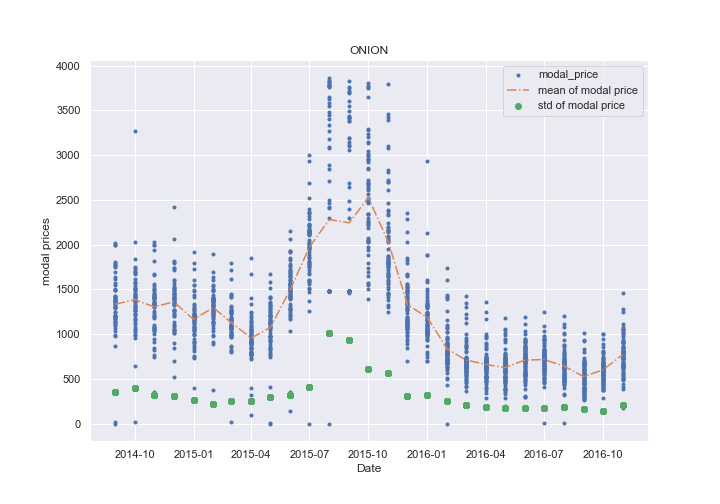
\includegraphics[width=13cm,keepaspectratio]{onion_mean_std.png}\\
	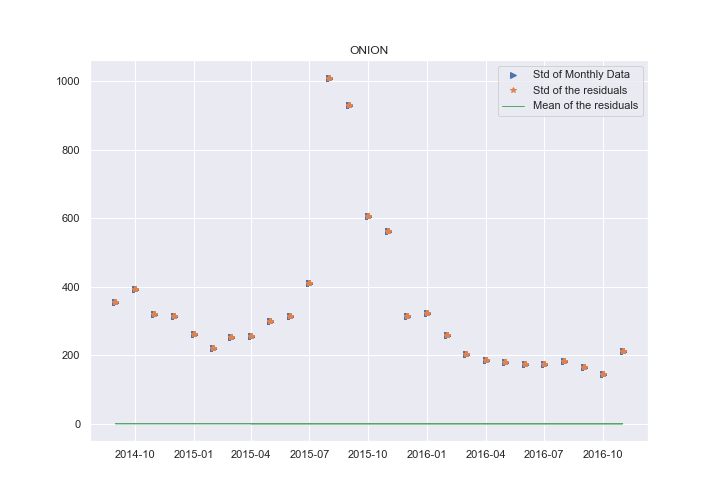
\includegraphics[width=13cm,keepaspectratio]{onion_std_resid}
	\caption{Top figure shows the data with its moving average and standard deviation. The bottom figure shows the mean and standard deviation after removing the overall trend under the assumption of additive seasonality and comparison of standard deviation before and after removing the overall trend.}
	\label{fig:onion_std}
\end{figure*}

\begin{figure*}
	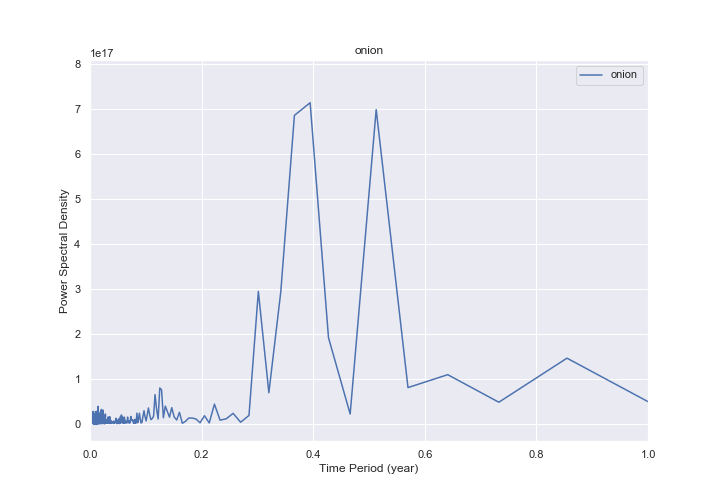
\includegraphics[width=12cm,keepaspectratio]{onion_before_spectrum.png}\\
	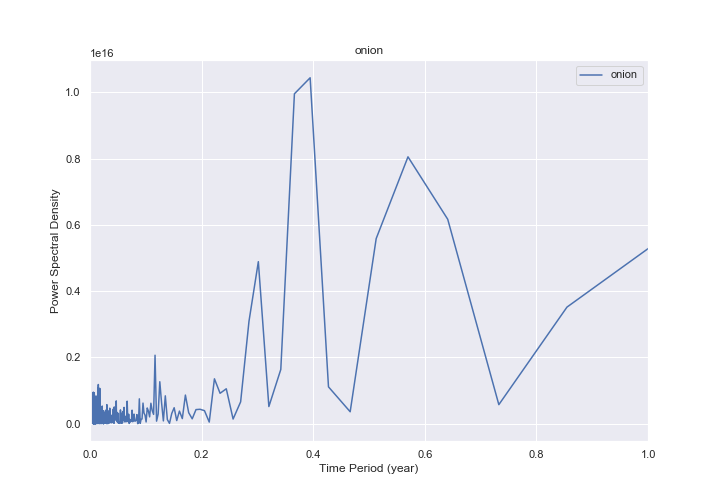
\includegraphics[width=12cm,keepaspectratio]{onion_after_spectrum.png}
	\caption{Spectrum of onion prices before and after removing overall trend. The frequencies have been suppressed by a factor of 10. }
	\label{fig:onion_spectrum}
\end{figure*}
\subsection{Multiplicative seasonality}

In the case of multiplicative seasonality, the residuals are denoted by:
\begin{equation}
R(t) = f(t) /(S(t)*Tr(t))
\end{equation}
Fig. \ref{fig:onion_multiplicative_residuals} shows the residuals left after removing the overall trend in a multiplicative fashion. The figure also shows and compare the standard deviation of the residuals and actual data. The mean and standard deviation have been made constant in the process. Further, spectrum shown in Fig. \ref{fig:onion_spectrum_multiplicative} show that the frequency components have been suppressed by a factor of $10^{14}$. This huge difference points to the multiplicative behavior of the seasonality in the prices.

\begin{figure*}
	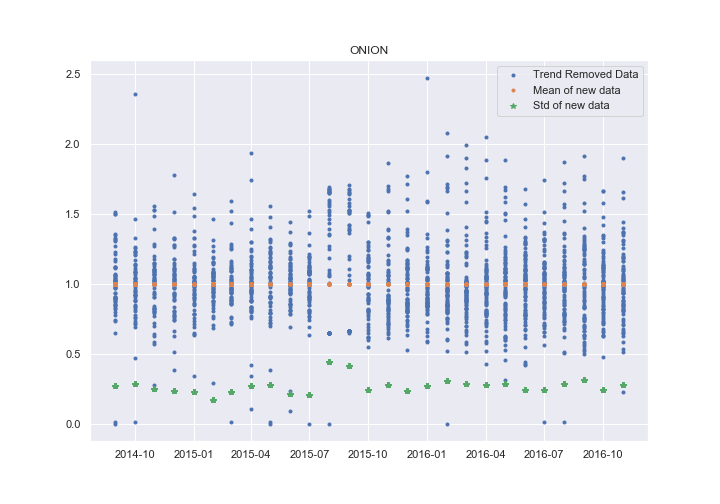
\includegraphics[width=12cm,keepaspectratio]{onion_resid_mean_std}\\
	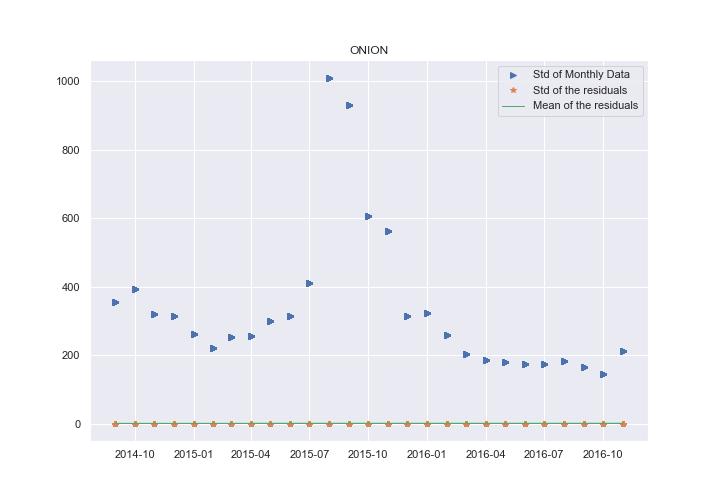
\includegraphics[width=12cm,keepaspectratio]{onion_std_resid_multi}
	\caption{Top figure shows the data with its moving average and standard deviation of the residuals after removing multiplicative seasonality. The bottom figure shows the comparison of standard deviation before and after removing the overall trend. }
	\label{fig:onion_multiplicative_residuals}
\end{figure*}
\begin{figure*}
	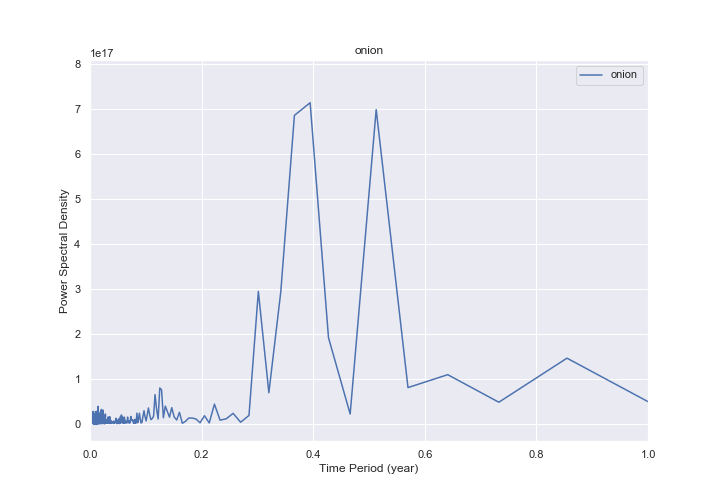
\includegraphics[width=12cm,keepaspectratio]{onion_before_spectrum.png}\\
	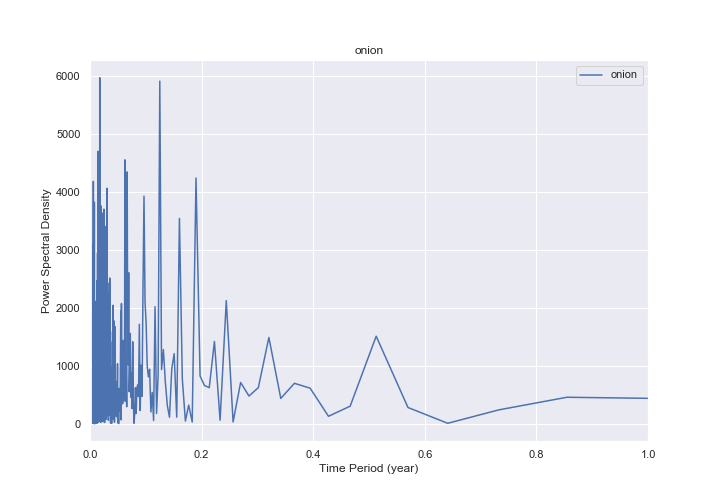
\includegraphics[width=12cm,keepaspectratio]{onion_before_spectrum_multi}
	\caption{Spectrum of onion prices before and after removing overall trend. The frequencies have been suppressed by a factor of $10^{14}$. }
	\label{fig:onion_spectrum_multiplicative}
\end{figure*}
\clearpage
\begin{figure}
	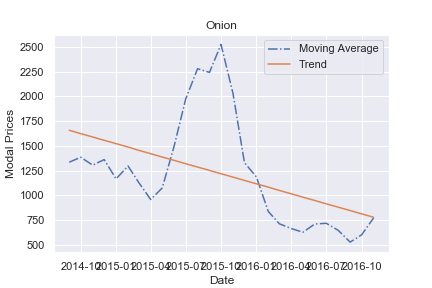
\includegraphics[width=15cm,keepaspectratio]{onion_trend.png}\\
	\caption{The trend component of the onion for time period 2014-16. }
	\label{fig:onion_trend}
\end{figure}
\subsection{Trend of prices and Seasonal Component}
In the previous section, argument was presented suggesting the presence of multiplicative seasonality. Since, the overall trend was shown to be a function of trend and seasonality, $OTr(t)$ can now be represented in the following manner:
\begin{equation}
	OTr(t) = Tr(t)*S(t)
\end{equation}
Thus the overall trend was decomposed into $Tr(t)$ and $S(t)$ which have been given below.

\begin{figure}

	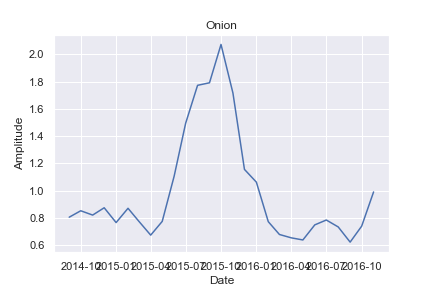
\includegraphics[width=15cm,keepaspectratio]{onion_seasonality.png}
	\caption{The seasonal component of the onion for time period 2014-16. }
	\label{fig:onionseasonal}
\end{figure}
\section{Future Work}
The work presented in the document dealt with data cleaning, exploration, trend and seasonality evaluation. An example case of onion was presented due to its importance for the Maharashtra Govt. The presented work will be followed by study and comparison of the APMC trends. Also, the minimum support price will be used to investigate the extent to which market price differs from the price at which farmers sold their product. In several articles, the overall trend presented in the document has been reported to repeat. This means, there is a huge scope of developing forecasting techniques around the available data and to forecast surge of prices and decrease in arrivals. A more investigative work would involve relating the data to the hoarding practices followed by the distributors and farmers. 
\section{Acknowledgement} 
The author thanks SocialCops team for providing this challenge. The entire challenge is very exciting and also eye opening. 
\end{document} 
